%
%  This is an example of how a LaTeX thesis should be formatted.  This
%  document contains chapter 1 of the thesis.
%
%  Time-stamp: "[sample-chapter1.tex] last modified by Scott Budge (scott) on 2017-01-12 (Thursday, 12 January 2017) at 10:20:50 on goga.ece.usu.edu"
%
%  Info: $Id: sample-chapter1.tex 998 2017-03-21 16:44:33Z scott $   USU
%  Revision: $Rev: 998 $
% $LastChangedDate: 2017-03-21 10:44:33 -0600 (Tue, 21 Mar 2017) $
% $LastChangedBy: scott $
%

\chapter{INTRODUCTION}
%%%%%%%% This line gets rid of page number on first page of text
\thispagestyle{empty}
%%%%%%%%%%%%%

Bioreactor design is a relatively complex engineering task, which is studied in the discipline of biochemical engineering. Under optimum conditions, the microorganisms or cells can perform their desired function with limited production of impurities. The environmental conditions inside the bioreactor, such as temperature, nutrient concentrations, pH, and dissolved gases (especially oxygen for aerobic fermentations) affect the growth and productivity of the organisms. The temperature of the fermentation medium is maintained by a cooling jacket, coils, or both. Particularly exothermic fermentations may require the use of external heat exchangers. Nutrients may be continuously added to the fermenter, as in a fed-batch system, or may be charged into the reactor at the beginning of fermentation. The pH of the medium is measured and adjusted with small amounts of acid or base, depending upon the fermentation. For aerobic (and some anaerobic) fermentations, reactant gases (especially oxygen) must be added to the fermentation. Since oxygen is relatively insoluble in water (the basis of nearly all fermentation media), air (or purified oxygen) must be added continuously. The action of the rising bubbles helps mix the fermentation medium and "strips" out waste gases, such as carbon dioxide. In practice, bioreactors are often pressurized; this increases the solubility of oxygen in water. In an aerobic process, optimal oxygen transfer is sometimes the rate limiting step.

\section{Specifications of a bioreactor}
A typical bioreactor shown in Fig~\ref{fig:split} consists of following parts:\newline
1.\textbf{Agitator} – used for the mixing of the contents of the reactor which keeps the “cells” in the perfect homogenous condition for better transport of nutrients and oxygen to the desired product(s).\newline
2.\textbf{Baffle} – used to break the vortex formation in the vessel, which is usually highly undesirable as it changes the center of gravity of the system and consumes additional power.\newline
3.\textbf{Sparger} – In aerobic cultivation process, the purpose of the sparger is to supply adequate oxygen to the growing cells.\newline
4.\textbf{Jacket} – The jacket provides the annular area for circulation of constant temperature of water which keeps the temperature of the bioreactor at a constant value.\newline


\begin{figure}[htbp]
\centering
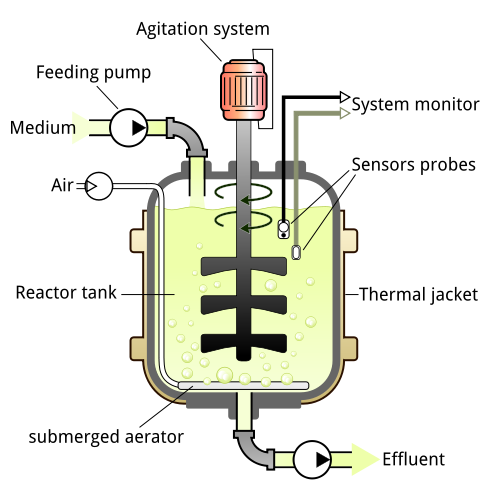
\includegraphics[width=0.7\textwidth]{images/reactor.png}
\caption{Bioreactor.}
\label{fig:split}
\end{figure}
\section{UASB reactor}
An efficient anaerobic digestion (AD) of organic matter is a result of a complex microbial interaction inside a bioreactor. For the high-rate anaerobic digestion of a feedstock, an up flow anaerobic sludge blanket reactor (UASB) is a common choice. 

UASB uses an anaerobic process whilst forming a blanket of granular sludge which suspends in the tank. Wastewater flows upwards through the blanket and is processed (degraded) by the anaerobic microorganisms. The upward flow combined with the settling action of gravity suspends the blanket with the aid of flocculates. The blanket begins to reach maturity at around three months. Small sludge granules begin to form whose surface area is covered in aggregations of bacteria. In the absence of any support matrix, the flow conditions create a selective environment in which only those microorganisms capable of attaching to each other survive and proliferate. Eventually the aggregates form into dense compact biofilms referred to as "granules".Biogas with a high concentration of methane is produced as a by-product, and this may be captured and used as an energy source, to generate electricity for export and to cover its own running power.

\begin{figure}[htbp]
\centering
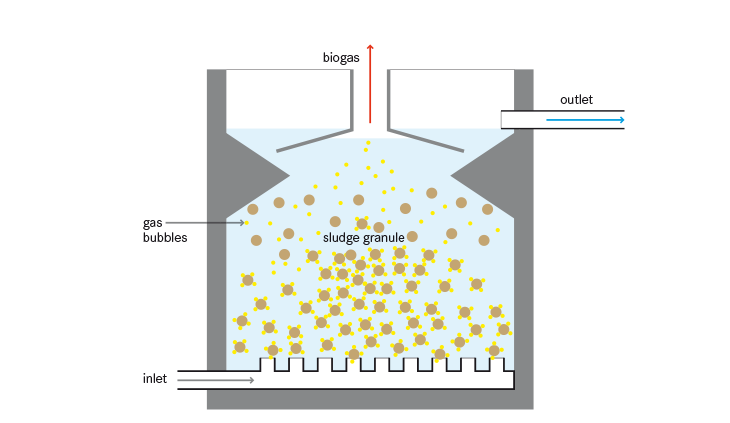
\includegraphics[width=1.0\textwidth]{images/usab.png}
\caption{A USAB reactor.}
\label{fig:usab reactor}
\end{figure}

\section{Background}

The predominant execution of this reactor is because of the specific association of microorganisms into circular granular structures. The process of granulation was first noticed and documented in the early 1980s[citation] and since then many anaerobic granulation theories have been presented. The main reasoning for the granulation per se is the up-flow velocity inside sludge bed of a UASB reactor. Microbial cells moving up with the flow of the feed tend to stick to the other microbial cells. Such sticking behavior prevents a washout of the microbial inoculum from a reactor since the outlet for the digested feed is in the top of the reactor [3,4]. The most widely accepted theory states that granulation starts with a formation of a future granules core, comprised of filamentous methanogenic bacteria Methanothrix, together with Methanosarcina, which secrete extracellular polymers (ECP) [citation]. The surface of this change and become attractive for the oppositely charged anaerobic bacteria that are present in the dispersed inoculum of a UASB[citation]. Chemo-attractancy of other bacteria towards ECPs and substrate around the granule core may also play a major role in the further aggregation and formation of mature granules [citation]. Despite these possible explanations of the granulation process, there is still no agreement on which of the possible theories correctly explain this most important and crucial role of granulation. The key factors of granulation are still to be determined, whether they are physical, biochemical or a combination of physicochemical properties of the cells and the way the organic matter transforms over space and time.

Bioaugmentation is a typical procedure in the field of wastewater treatment, utilized to acquaint another metabolic capacity with either oxygen consuming or anaerobic granules. In this study, we have created a simulation model which is concerned about digesting celloboise, as a major component of microalgae in a bioreactor. Once a mature granule is formed, protein lipid is used as an alternative substrate that will be supplied to a mature granule. Protein, being a main component of cyanobacteria, will promote growth and incorporation of a cell type that can degrade protein (selective pressure). 

Some exploration additionally proposes a requirement for a tight biochemical collaboration to happen between the bioaugmented strain and the available intact community (Citation). Such biochemical interaction together with substrate niche availability will lead to a stratification or compartmentalization of the bioaugmented strain in the granule. Intending to reveal insight to the systems of the anaerobic granulation, current group of metabolic and biochemical cooperations amid bioaugmentation of anaerobic granules can be connected to build up a prescient demonstrate for the bioaugmented granule. A model that can outwardly illustrate shifting stratifications of various trophic microbial gatherings will be of assistance for the designers and scientists, who are working both research center and modern scale anaerobic digesters and wish to improve reactor execution. In the past work, a model of anaerobic granulation was effectively manufactured, and a search engine was utilized to locate the ideal methane generation from the glucose concentration of COD corresponding to the low-strength wastewaters (Doloman et al., 2017). 

\section{Current biological model}

The new model reported here builds up on the basic principles of de novo anaerobic granulation reported earlier and a more complex model is suggested. Described granule formation is based on the aerobic decomposition of cellulose, thus describing a more vigorous microbial network of 5-6 different bacteria. To simulate bioaugmentation process as in the lab anaerobic digesters, new additional bacterial species are introduced to the mature complex granule, together with a specific substrate that can only be decomposed by the new introduced bacterium. Cellulose, being a main carbohydrate component of all plant and algal biomass, was chosen as a substrate of interest due to its relatively complex anaerobic digestion scheme, allowing multiple trophic groups to occupy the same layer in the granule. Lipid derivative was chosen as a substrate of interest that would be degraded with the simulated bioaugmented granule. This derivative, oleate is usually produced as an intermediate from anaerobic degradation of lipids, by glycerol-fermenting acidogenic bacteria (Angleidaki, 1988). Oleate is introduced into the model together with an arbitrary oleate degrading bacterium, providing a full contrast to the decomposition of the cellulose substrate and thus bioaugmenting the granule with the new or additional metabolic capability. Thus, the purpose of this study was to model different scenarios of bioaugmenting anaerobic granule with the novel microbial species: with and without pressure of the available specific substrate.

\begin{figure}[htbp]
\centering
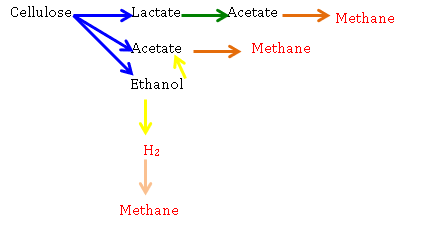
\includegraphics[width=0.7\textwidth]{images/schema1.png}
\caption{Schema of complex granule formation.}
\label{fig:Schema of complex granule formation}
\end{figure}

Current study explores different scenarios of bioaugmenting anaerobic granules with the novel microbial species: with and without pressure of the available specific substrate. The general aim of the study is to expand the knowledge on both successful bioaugmentation experiments and inspire for industrial-scale modifications in anaerobic digestion processes. 

% Please add the following required packages to your document preamble:
% \usepackage[table,xcdraw]{xcolor}
% If you use beamer only pass "xcolor=table" option, i.e. \documentclass[xcolor=table]{beamer}
\begin{table}
\centering
\caption{Microbe responsible for the conversion pathway}
\label{table1}
\begin{tabular}{|l|l|}
\hline
Conversion pathway                                       & Type of microbe responsible \\ \hline
{\color[HTML]{00009B} \textbf{------------\textgreater}} & Clostridium I               \\ \hline
{\color[HTML]{32CB00} \textbf{------------\textgreater}} & Clostridium II              \\ \hline
{\color[HTML]{036400} \textbf{------------\textgreater}} & Methanogen I                \\ \hline
{\color[HTML]{FFC702} \textbf{------------\textgreater}} & Desulfovibrio               \\ \hline
{\color[HTML]{38FFF8} \textbf{------------\textgreater}} & Methanogen II               \\ \hline
{\color[HTML]{FE0000} \textbf{------------\textgreater}} & OleateDegrader              \\ \hline
\end{tabular}
\end{table}


